\chapter{Evaluation}\label{cha:evaluation}

Envoy is designed based on assumptions about a platform that does not yet exist. This limits how the system can be evaluated in two ways. The first is scalability. While common bottlenecks can be avoided and the architecture examined for potential scalability limitations, a system without a large-scale implementation can never be fully tested for issues that only appear at large scales. The best that can be achieved is to identify the most likely sources of problems and extrapolate the results of testing on a smaller scale. The architecture can also be evaluated against assumptions about the workloads it is intended to support, which leads to the second limitation: workloads cannot be accurately forecast. Predicting and simulating client access patterns is a difficult problem even for existing environments \cite{ganger95}, and the problem is amplified for service clusters. As a general purpose platform, service clusters are intended to support a wide range of existing workloads and to enable a flourishing ecosystem of computation services that create entirely new workloads. The design and the evaluation must necessarily rely on assumptions about how the system will be used, and those assumptions limit the applicability of the results.

In this chapter I evaluate the Envoy prototype with three principal goals: to measure the impact of specific design choices, including the basic distributed organisation and cache layout, to assess the scalability of the system, and to evaluate Envoy's ability to support the types of workloads expected in service clusters.

\section{Methodology}

The absence of a realistically sized service cluster limits the scope of system-level testing and the usefulness of many application-level results. The performance side-effects of interacting components and the access patterns of different clients are particularly difficult to predict. The performance characteristics of the storage layer depend on design elements and implementation choices beyond the scope of this dissertation. These factors combined with the poor public availability of many comparable systems limit direct comparisons to previous work.

Building and evaluating a prototype of the Envoy file system is not a futile exercise, however. The artefact may reveal little about real-world usage and behaviour, but measuring it can still do much to justify or condemn the design. This section starts by outlining assumptions about service clusters that influence the design, how the design reflects them, and how measuring the prototype helps to evaluate the decisions made. It concludes with a description of the testing environment and the benchmarks used.

\subsection{Assumptions and goals}

Envoy's success in achieving its stated goals is evaluated partly through argument and comparison to other work as described in previous chapters. Other aspects can be tested directly on a small installation and the results extrapolated to larger configurations. While not comprehensive, this approach is consistent with Envoy's role as one part of a complete service cluster environment. Further research and engineering will be necessary before service clusters can be fully evaluated on their own merits. Some of the assumptions that underpin them can be tested directly, while others must rest on arguments and an appeal to past and future work.

\subsubsection{Independent clients}

Though efficient sharing is important, individual clients accessing unshared data dominates most workloads. Even when data sets overlap, time may divide access from different clients, effectively yielding exclusive access that is transferred from one client to the next over time. Envoy seeks to capture these patterns by subdividing territories to distribute file ownership and control, and by dynamically updating the boundaries over time in response to changing usage. When this is successful, or when access to was exclusive in the first place, Envoy resembles a simple client-server system serving files from an administrative virtual machine to a client virtual machine on the same host.

Since one of Envoy's goals is to create this intra-host configuration whenever possible, the evaluation starts by considering system performance under this circumstance. Maximizing raw performance is not the focus of the prototype implementation, but comparing it to systems with a similar topology creates baseline expectations for a production system, and examining absolute performance figures helps confirm the sanity of the overall design.

\secref{sec:independent-clients} evaluates the performance of Envoy as a file server within a single host. Composite performance numbers are compared to other client-server systems, and tests using different configurations help to demonstrate where performance costs are embedded in Envoy. In addition, performance for remote hosts is evaluated to show that the drive to localize traffic benefits performance as well as scalability.

\subsubsection{Shared images}

\secref{sec:shared-images} turns the evaluation to shared data. The emphasis of this section is not on performance---which is dependent largely on runtime topology as evaluated in \secref{sec:independent-clients} and the quality of the implementation---but rather on the behaviour of the system under shared workloads. In effect, \secref{sec:shared-images} evaluates Envoy's ability to localize traffic, and \secref{sec:independent-clients} explores the benefits and costs that result from its success or failure.

Some aspects of Envoy's dynamic behaviour cannot be adequately tested in the limited environment available for this evaluation. The Envoy design prizes simplicity and stability in the layout of territories, both to simplify testing and recovery, and to encourage cache sharing even in the presence of runtime conflicts. The latter goal is achieved by delaying territory transfers until traffic is clearly dominated by a remote participant or until a more slight imbalance has persisted for a longer period of time. Resisting change allows the cache on the owning host to serve all participants at the expense of a network hop from the remote client to the envoy. Rearranging boundaries more eagerly may reduce network hops, but it creates some migration latency and the new host may have to prime its cache before service can resume at full speed.

While the parameters controlling dynamic behaviour can be configured, the ideal balance of stability and layout optimality can only be adequately determined with realistic workloads. Oscillating demand could be best handled by reacting quickly and varying the territory layout in lock-step with traffic changes, or being reluctant to change in order to maximize cache efficacy on one of the hosts may prove better. In the absense of a larger test system and realistic workloads to evaluate specific parameters, this evaluation relies on artificial traffic loads that can be controlled and varied to test the response of the system.

\subsubsection{Scalability}

Envoy's scalability is not evaluated directly. To do so convincingly would require a large cluster with a diverse client base, and direct testing on a reduced scale would prove little. The presumed scalability of the system depends on successfully localizing as much traffic as possible. If all requests are satisfied by the same physical machine that hosts the client, then a cluster's capacity to host clients grows linearly with the number of machines added to the system. If most requests are handled locally and neighbouring hosts are consulted mainly to resolve runtime conflicts, then scalability is limited primarily by the degree of runtime sharing. Envoy's goal of scalability is based on a design that attempts to approximate that limit.

The storage layer is another source of traffic and inter-host dependence, but it is not fully specified in this work and cannot be evaluated fairly. A large persistent cache on each host reduces the direct load on the storage layer just as it did for AFS \cite{satyanarayanan85}, but by coupling storage nodes with clients hosts and using switched networking, the overall transaction capacity of the storage layer should scale with the number of hosts anyway, and the number of hosts limits the number of clients. The systems considered in \secref{sec:storage-layer-systems} have already demonstrated the scalability of similar storage architectures; conflict management and the coordination of metadata differentiate each system, but in Envoy that burden is not left to the storage layer.

\subsection{Test environment}

\subsubsection{Hardware}

\subsubsection{Benchmarks}

Linux source tree: stats about it

untar -- write test

tar > /dev/null -- read test

rsync -- 2nd read test

Bonnie: info about it

\section{Independent clients}\label{sec:independent-clients}

Much of the complexity in distributed file system design is related to data sharing, but sharing is less common than individual clients accessing private data. A service derived from a standalone machine typically requires a private boot image, and lightweight fork operations in Envoy encourage the cloning of entire images for private use by related and unrelated service instances.

To succeed as a distributed file system on a large scale, Envoy must provide a useful service to isolated clients that obviates the need for additional storage services for most clients. While there is no technical or administrative distinction between private and shared images, Envoy's design and runtime behaviour under these two conditions can be evaluated seperately. This section focuses on Envoy's performance and behaviour in the absense of sharing.

\subsection{Performance}

The prototype is not optimized, and absolute performance is not the focus of this evaluation. Nevertheless, it is helpful to establish baseline performance numbers to show that Envoy is viable as a file system. For context, the results are compared to \texttt{npfs}, a multi-threaded userspace 9p server, and \texttt{unfsd}, a single-threaded userspace NFS server. Userspace servers have additional overhead when compared to kernel implementations, but the penalty is assumed to be similar for all of the implementations tested. Standard benchmarks do a poor job of isolating the costs involved in Envoy's data paths, and most of the evaluation in this chapter eschews them in favor of more controlled tests, but this section starts with the Bonnie benchmark to provide some raw performance figures comparable to those from other systems.

\begin{figure}[t]
\centering
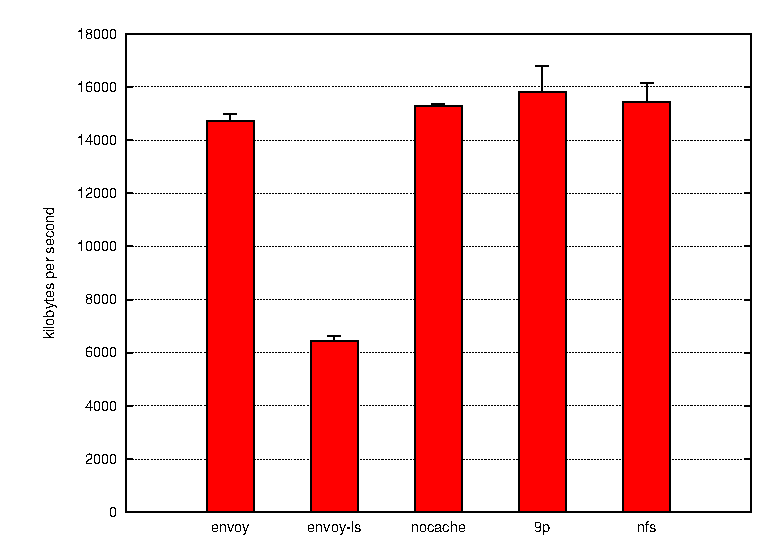
\includegraphics[width=\figwidth]{figures/bonnie-druid1-write}
\caption[Bonnie benchmark results for block writes]{Bonnie benchmark results for block writes on a 2GB dataset. Results for Envoy, Envoy using a local storage server instance, Envoy with no persistent cache, a userspace 9p server, and a userspace NFS server are compared. Error bars show the standard deviation over ten runs.}
\label{fig:bonnie-druid1-write}
\end{figure}

\figref{fig:bonnie-druid1-write} shows the block write results of the Bonnie benchmark on a 2GB dataset. The four clusters show different client locations. druid-0 hosts the envoy that owns the territory for the Envoy results (displayed with and without the persistent cache enabled), and runs the server for the 9p and nfs results. druid-1 is a client VM on the same machine, skiing-0 the administrative VM on a remote machine (which also hosts an envoy instance), and skiing-1 is a client domain on the remote machine. Both druid-0 and skiing-0 host storage server instances with complete replicas of all storage objects.

Envoy's persistent cache creates a large penalty for writes, but this is a worst-case result. Data must be written twice since a storage instance is located on the same machine using the same hard drive, in addition to the storage replica on the skiing-0. Disabling the persistent cache boosts write performance considerably, putting it on par with the other servers. Writing it twice on two machines incurs some overhead, but it is acceptable for the simplistic storage server used in the prototype. 9p is generally a bit faster than NFS because of its simpler protocol and larger message size, but in this simple test waiting for the disk dominates all of the servers.

\begin{figure}[t]
\centering
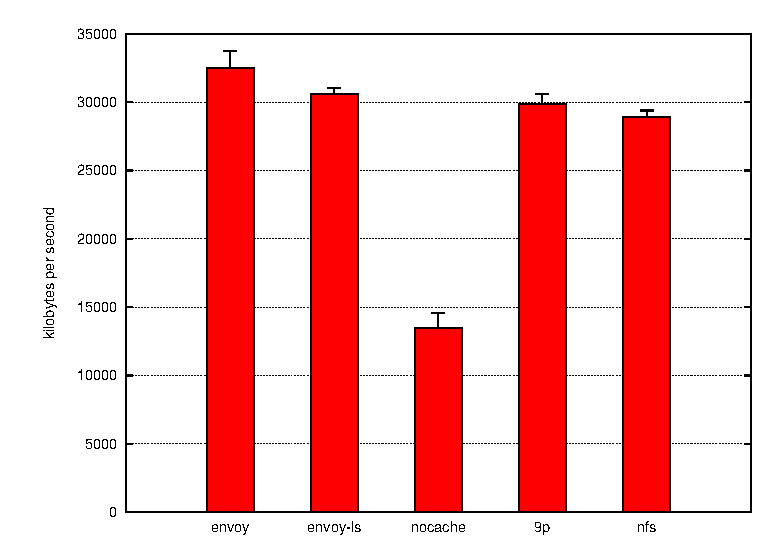
\includegraphics[width=\figwidth]{figures/bonnie-druid1-read}
\caption[Bonnie benchmark results for block reads]{Bonnie benchmark results for block reads on a 2GB dataset. Results for Envoy, Envoy using a local storage server instance, Envoy with no persistent cache, a userspace 9p server, and a userspace NFS server are compared. Error bars show the standard deviation over ten runs.}
\label{fig:bonnie-druid1-read}
\end{figure}

\figref{fig:bonnie-druid1-read} shows the block read results from the same benchmark. The persistent cache does not incur a double-access penalty as in the write case, so it improves the results. All data is present in the persistent cache (though the dataset is too large for the in-memory cache), so the Envoy results are similar to the 9p results in this test. Disabling the persistent cache forces retrieval from the storage servers, and each request is randomly directed to one of the two replicas.

The NFS numbers are more confusing. This is probably due to the interactions between the client-side cache and the server cache. The cache was flushed before each run by deleting all files and remounting the partition, the server processes were restarted, and clients were remounted, but each run of the benchmark executes a series of tests in succession without any explicit \texttt{sync} calls. The interaction of two levels of delayed write-back caching, particularly when both are part of the same buffer cache on druid-0, could explain the curious results. The behaviour of NFS is not the focus of this evaluation, however.

\begin{figure}[t]
\centering
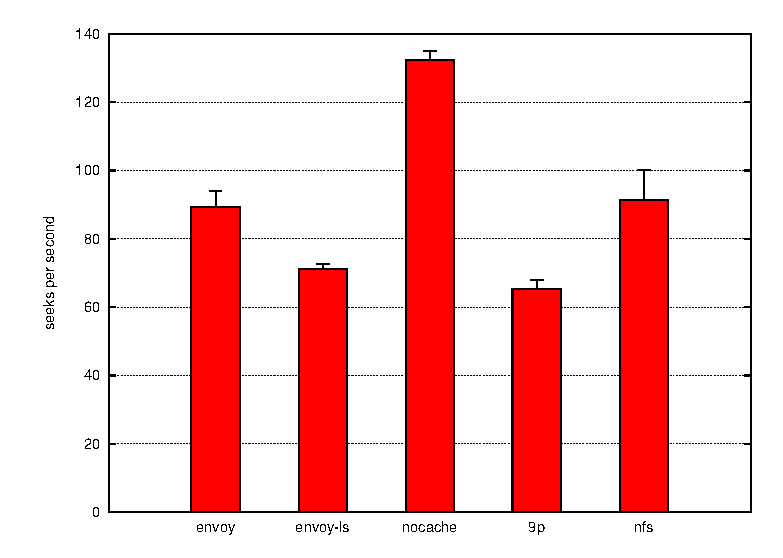
\includegraphics[width=\figwidth]{figures/bonnie-druid1-seek}
\caption[Bonnie benchmark results for random seeks]{Bonnie benchmark results for random seeks on a 2GB dataset. Results for Envoy, Envoy using a local storage server instance, Envoy with no persistent cache, a userspace 9p server, and a userspace NFS server are compared. Error bars show the standard deviation over ten runs.}
\label{fig:bonnie-druid1-seek}
\end{figure}

\figref{fig:bonnie-druid1-seek} shows the results of the concurrent random seek test in Bonnie. Disabling the persistent cache helps Envoy because concurrent requests are randomly directed to two different disks, and the effective cache size is much larger. With no persistent cache, the memory on druid-0 and skiing-0 is used mostly by the storage server cache, but when the persistent cache is enabled, only druid-0 contributes memory and it is split between its storage instance and the persistent cache. The prototype only allows one outstanding request per storage object, so seek penalties are not significantly reduced by using two disks. NFS probably also benefits from combining the client-side cache with the server cache. In Envoy's intended environment, client cache sizes would be smaller and server caches larger to encourage sharing, but this benchmark only acts from a single client.

\subsection{Architecture}\label{sec:architectural-costs}

An important goal of the Envoy design is to localize data and metadata control when possible, and minimize the involvement of disinterested nodes when not possible. Private images are always controlled by the envoy instance on the same machine as the client using it, and territories in shared images are managed by the most active participant. Besides reducing collateral impact in a bid to improve scalability, localizing control and caching has direct performance benefits for clients.

As described in \secref{sec:data-paths}, requests follow one of several paths to completion depending on whether or not the required data is cached and whether ownership is local or remote. The worst case for local or remote ownership is when the data must be retrieved from the storage layer.


If the goal is to get stuff as local as possible, quantify the benefits of achieving that. Measure the overheads of data paths and cache decisions.

\subsubsection{Local impact}

Independence of private images

\subsection{Cache}

\subsubsection{Quantifying sharing}\label{sec:quantifying-sharing}

SUSE10 upgrade, install services

compare image overlap

boot two related images (one cold and other warm) and compare with the same test for identical images

show sharing: boot one VM from cold cache, boot another based on same template

\section{Shared images}\label{sec:shared-images}



\subsection{Territory migration}

cost of transferring state

two machines with kernel in hot cache, do read test while transferring ownership back and forth between them

\subsection{Dynamic behaviour}

Test dynamic territory management, less about performance than behaviour

probabilistic traffic driven to overlapping areas

shared image with (independent) home directories

2 log files in one directory

producer-consumer

\subsubsection{Sharing application}
something that shares in a complex but predictable fashion

\section{Image operations}

\subsubsection{Forks}

cheap and fast---these always happen from a read-only snapshot

\subsubsection{Snapshots}

single territory

untar the kernel while a bunch of snapshots happen and measure the impact

snapshots with many territories

\section{Summary}
